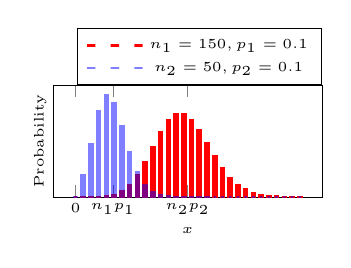
\begin{tikzpicture}
    % \pgfplotsset{ticks = none}
    \tiny
    \begin{axis}[
            xlabel={$x$},
            ylabel={Probability},
            legend style={at={(1,1)},anchor=south east},
            legend style={font=\tiny},
            ymin  = 0,
            xtick={0,5,15},
            xticklabels={0,$n_1p_1$,$n_2p_2$},
            ytick = \empty,
            yticklabel=\empty,
            height = 3cm,
            width = 5cm,
            grid style=dashed,
            bar width=1pt,
        ]
        \addplot [
            domain=0:30,
            samples=30,
            color=red,
            ybar,
            draw opacity=1,
            line width = 1pt,
        ]
        {factorial(150)/(factorial(x)*factorial(150-x))*(0.1^x)*((0.9)^(150-x))};
        \addlegendentry{$n_1=150, p_1=0.1$}

        \addplot [
            domain=0:30,
            samples=30,
            color=blue,
            ybar,
            draw opacity=0.5,
            line width = 1pt,
        ]
        {factorial(50)/(factorial(x)*factorial(50-x))*0.1^x*(0.9)^(50-x)};
        \addlegendentry{$n_2=50,p_2=0.1$}
    \end{axis}
\end{tikzpicture}